% Editable native annotations around unchanged verified IDE photographs.
\par
\begin{figure}[htbp]
\centering
\newsavebox{\MARSmatmulzeroregistersBox}
\sbox{\MARSmatmulzeroregistersBox}{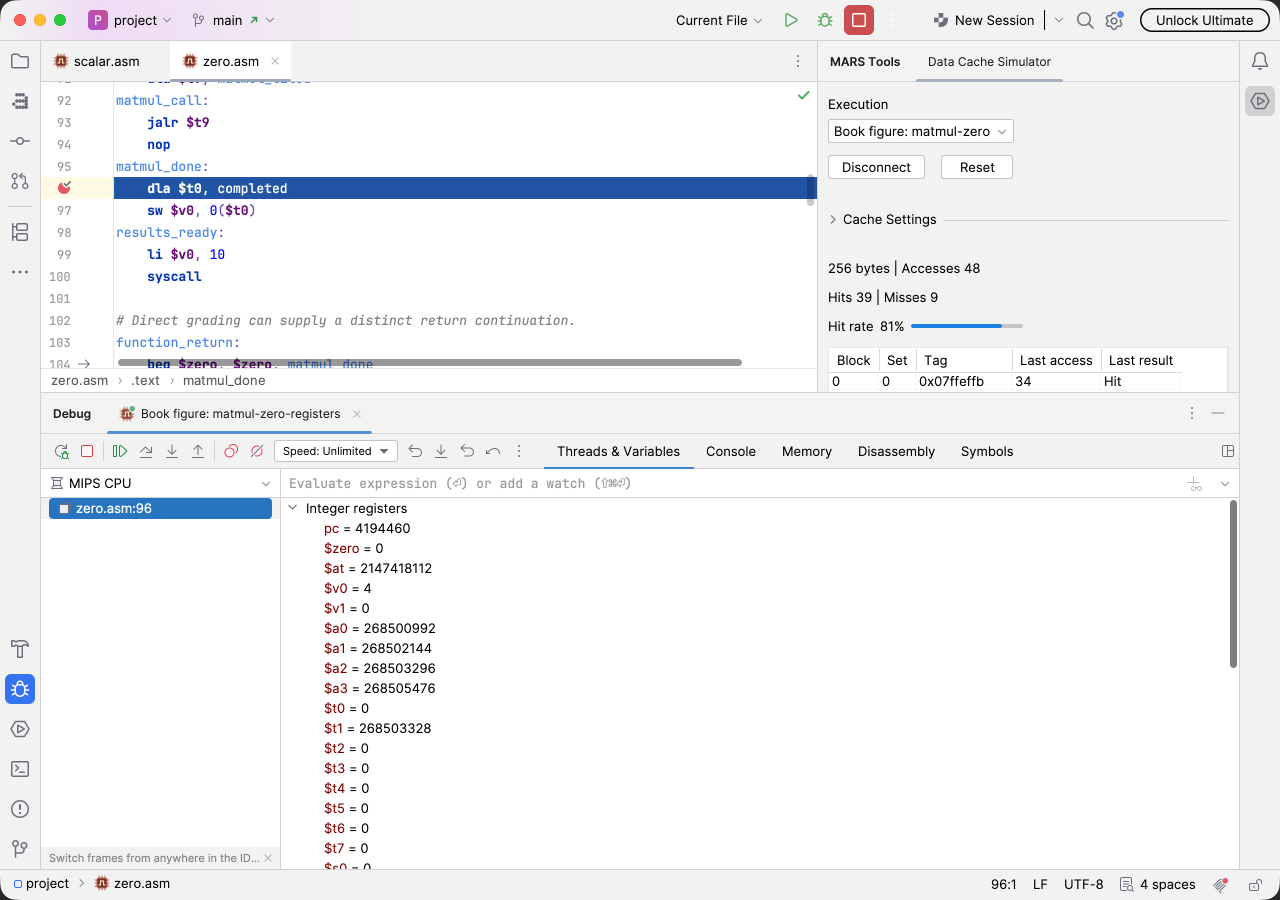
\includegraphics[artifact]{packages/022-blocked-matmul/captures/f02/registers.png}}
\newsavebox{\MARSmatmulzeroproductBox}
\sbox{\MARSmatmulzeroproductBox}{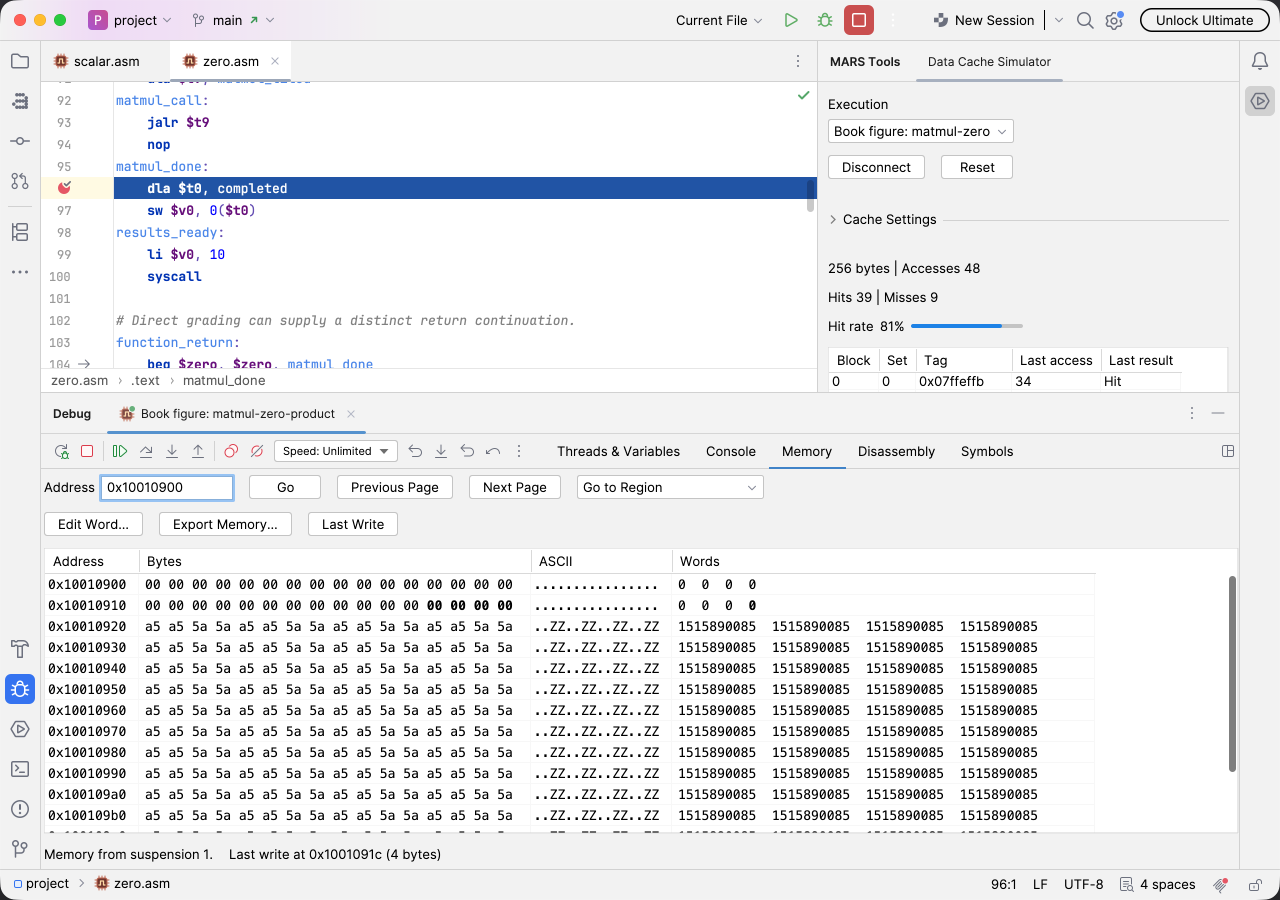
\includegraphics[artifact]{packages/022-blocked-matmul/captures/f02/product.png}}
\newsavebox{\MARSmatmulzerocallerBox}
\sbox{\MARSmatmulzerocallerBox}{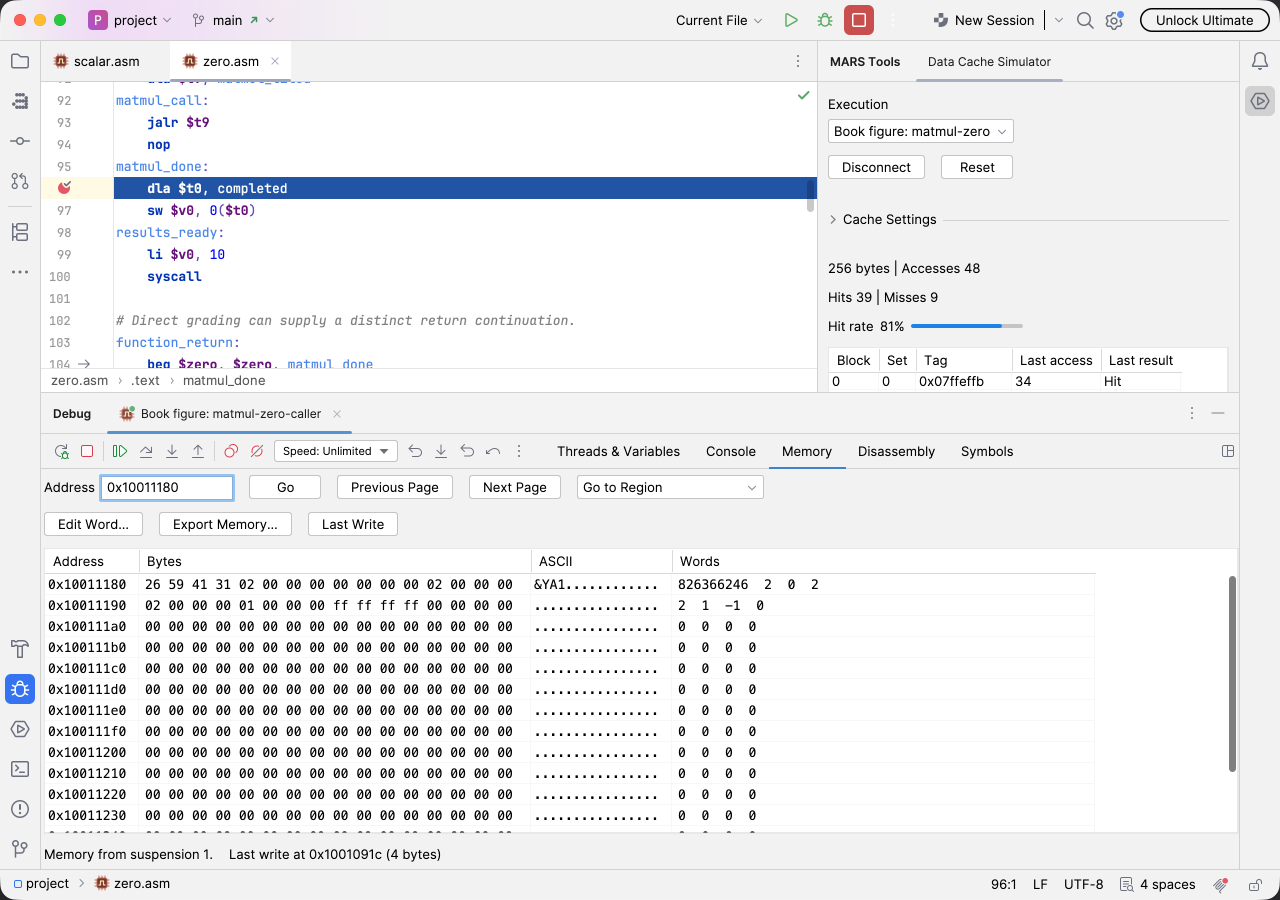
\includegraphics[artifact]{packages/022-blocked-matmul/captures/f02/caller.png}}
\edef\MARSmatmulzerosourceLeft{\the\dimexpr0.036718750\wd\MARSmatmulzeroregistersBox\relax}
\edef\MARSmatmulzerosourceBottom{\the\dimexpr0.774444444\ht\MARSmatmulzeroregistersBox\relax}
\edef\MARSmatmulzerosourceRight{\the\dimexpr0.713281250\wd\MARSmatmulzeroregistersBox\relax}
\edef\MARSmatmulzerosourceTop{\the\dimexpr0.170000000\ht\MARSmatmulzeroregistersBox\relax}
\edef\MARSmatmulzeroregistersLeft{\the\dimexpr0.246093750\wd\MARSmatmulzeroregistersBox\relax}
\edef\MARSmatmulzeroregistersBottom{\the\dimexpr0.334444444\ht\MARSmatmulzeroregistersBox\relax}
\edef\MARSmatmulzeroregistersRight{\the\dimexpr0.553906250\wd\MARSmatmulzeroregistersBox\relax}
\edef\MARSmatmulzeroregistersTop{\the\dimexpr0.640000000\ht\MARSmatmulzeroregistersBox\relax}
\edef\MARSmatmulzeroproductLeft{\the\dimexpr0.034375000\wd\MARSmatmulzeroproductBox\relax}
\edef\MARSmatmulzeroproductBottom{\the\dimexpr0.311111111\ht\MARSmatmulzeroproductBox\relax}
\edef\MARSmatmulzeroproductRight{\the\dimexpr0.584375000\wd\MARSmatmulzeroproductBox\relax}
\edef\MARSmatmulzeroproductTop{\the\dimexpr0.608888889\ht\MARSmatmulzeroproductBox\relax}
\edef\MARSmatmulzerocallerLeft{\the\dimexpr0.034375000\wd\MARSmatmulzerocallerBox\relax}
\edef\MARSmatmulzerocallerBottom{\the\dimexpr0.311111111\ht\MARSmatmulzerocallerBox\relax}
\edef\MARSmatmulzerocallerRight{\the\dimexpr0.584375000\wd\MARSmatmulzerocallerBox\relax}
\edef\MARSmatmulzerocallerTop{\the\dimexpr0.608888889\ht\MARSmatmulzerocallerBox\relax}
\begin{tikzpicture}[alt={Four annotated details at matmul_done show return four, four zero result doublewords, shape two zero two two, tiled method one and completed still minus one. The exact checked access stream has no input reads.}]
\node[anchor=north west,inner sep=0,font=\small\bfseries] (source-title) at (6mm,0) {Next instruction at this boundary};
\node[anchor=north west,inner sep=0] (source) at ([yshift=-1mm]source-title.south west) {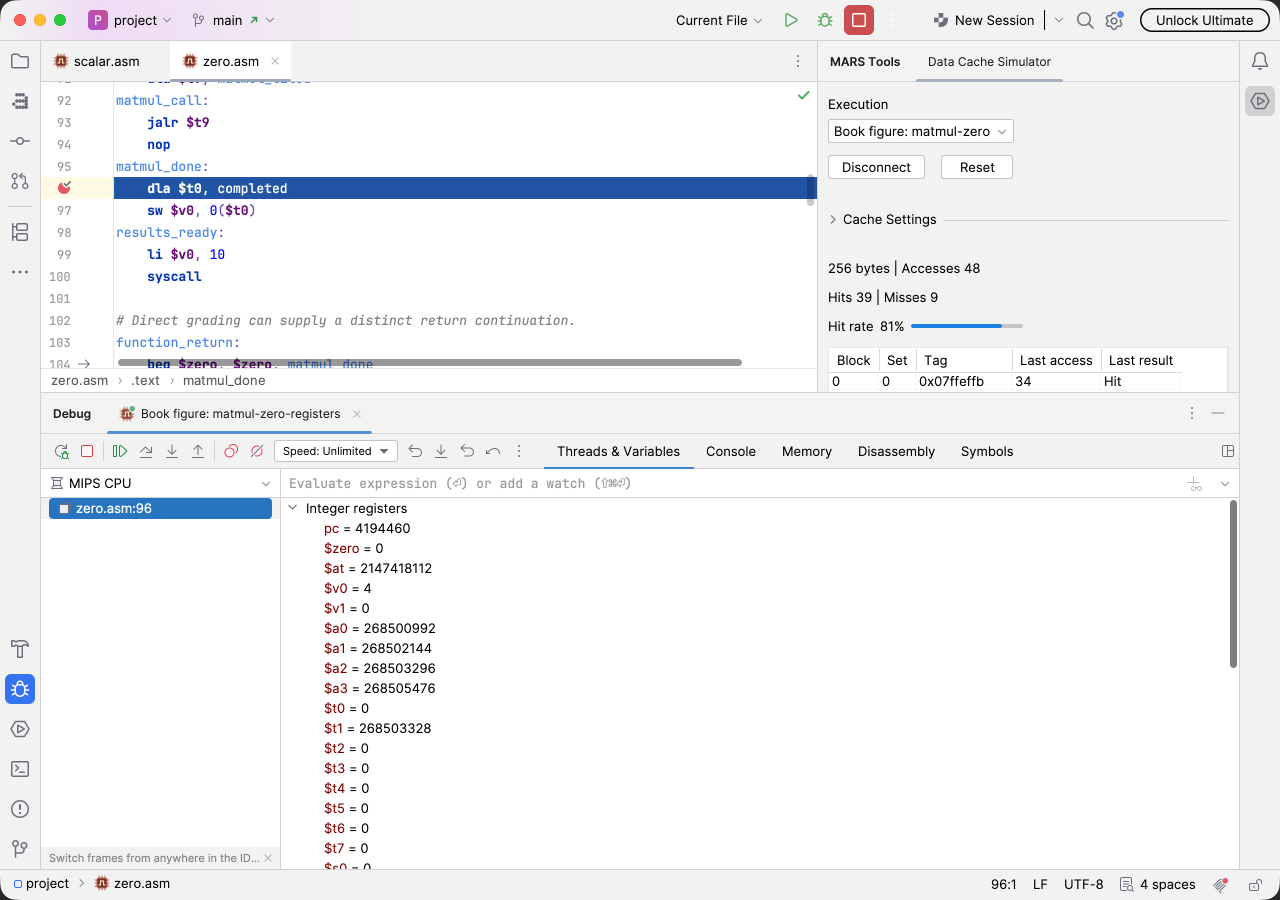
\includegraphics[width=0.54\linewidth,artifact,trim={\MARSmatmulzerosourceLeft{} \MARSmatmulzerosourceBottom{} \MARSmatmulzerosourceRight{} \MARSmatmulzerosourceTop{}},clip]{packages/022-blocked-matmul/captures/f02/registers.png}};
\begin{scope}[shift={(source.south west)},x={($(source.south east)-(source.south west)$)},y={($(source.north west)-(source.south west)$)}]
\draw[black,line width=0.7pt] (0.215625000,0.080000000) rectangle (0.750000000,0.520000000);
\node[draw=black,fill=white,circle,inner sep=1.5pt,font=\footnotesize] at ($(0.215625000,0.520000000)+(-3mm,0)$) {1};
\end{scope}
\node[anchor=north west,inner sep=0,font=\small\bfseries] (registers-title) at (0.58\linewidth,0 |- source-title.north) {Register value at this boundary};
\node[anchor=north west,inner sep=0] (registers) at ([yshift=-1mm]registers-title.south west) {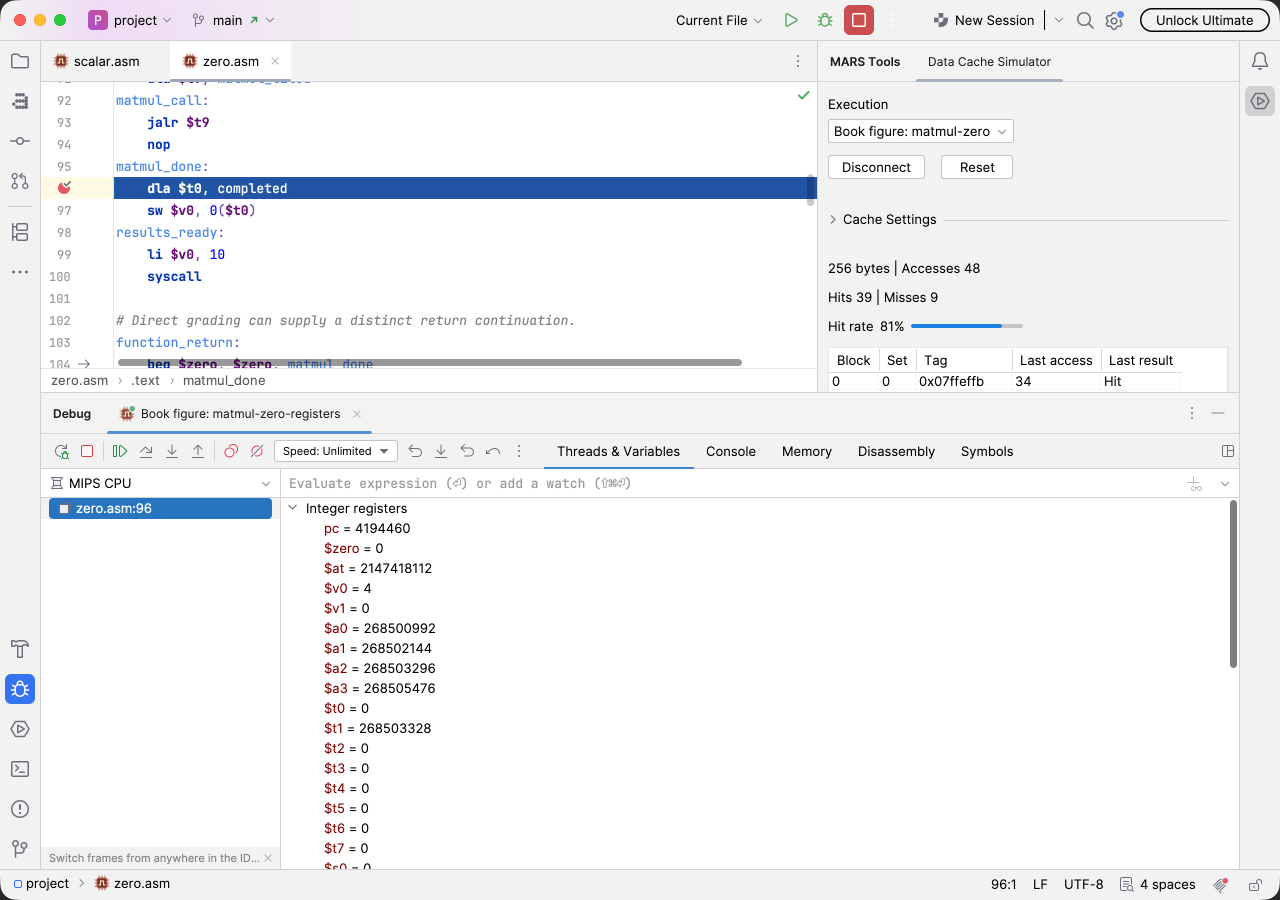
\includegraphics[width=0.42\linewidth,artifact,trim={\MARSmatmulzeroregistersLeft{} \MARSmatmulzeroregistersBottom{} \MARSmatmulzeroregistersRight{} \MARSmatmulzeroregistersTop{}},clip]{packages/022-blocked-matmul/captures/f02/registers.png}};
\begin{scope}[shift={(registers.south west)},x={($(registers.south east)-(registers.south west)$)},y={($(registers.north west)-(registers.south west)$)}]
\draw[black,line width=0.7pt] (0.023437500,0.043478261) rectangle (0.226562500,0.913043478);
\node[draw=black,fill=white,circle,inner sep=1.5pt,font=\footnotesize] at ($(0.023437500,0.913043478)+(-3mm,0)$) {2};
\end{scope}
\node[anchor=north west,inner sep=0,font=\small\bfseries] (product-title) at ([yshift=-1mm]source.south west) {Output doublewords};
\node[anchor=north west,inner sep=0] (product) at ([yshift=-1mm]product-title.south west) {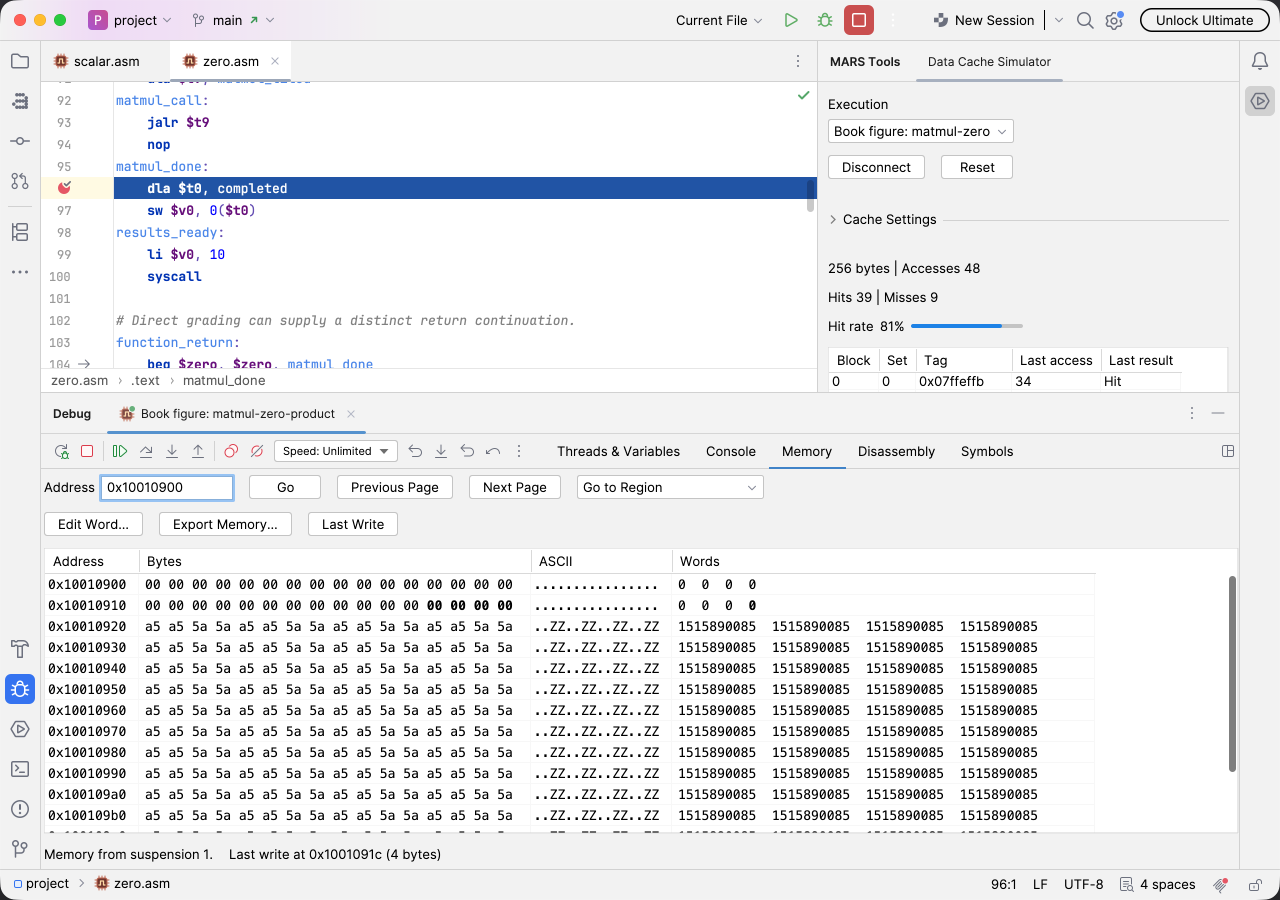
\includegraphics[width=0.84\linewidth,artifact,trim={\MARSmatmulzeroproductLeft{} \MARSmatmulzeroproductBottom{} \MARSmatmulzeroproductRight{} \MARSmatmulzeroproductTop{}},clip]{packages/022-blocked-matmul/captures/f02/product.png}};
\begin{scope}[shift={(product.south west)},x={($(product.south east)-(product.south west)$)},y={($(product.north west)-(product.south west)$)}]
\draw[black,line width=0.7pt] (0.194672131,0.055555556) rectangle (0.997950820,0.638888889);
\node[draw=black,fill=white,circle,inner sep=1.5pt,font=\footnotesize] at ($(0,0.638888889)+(-3mm,0)$) {3};
\end{scope}
\node[anchor=north west,inner sep=0,font=\small\bfseries] (caller-title) at ([yshift=-1mm]product.south west) {Shape, method and saved count};
\node[anchor=north west,inner sep=0] (caller) at ([yshift=-1mm]caller-title.south west) {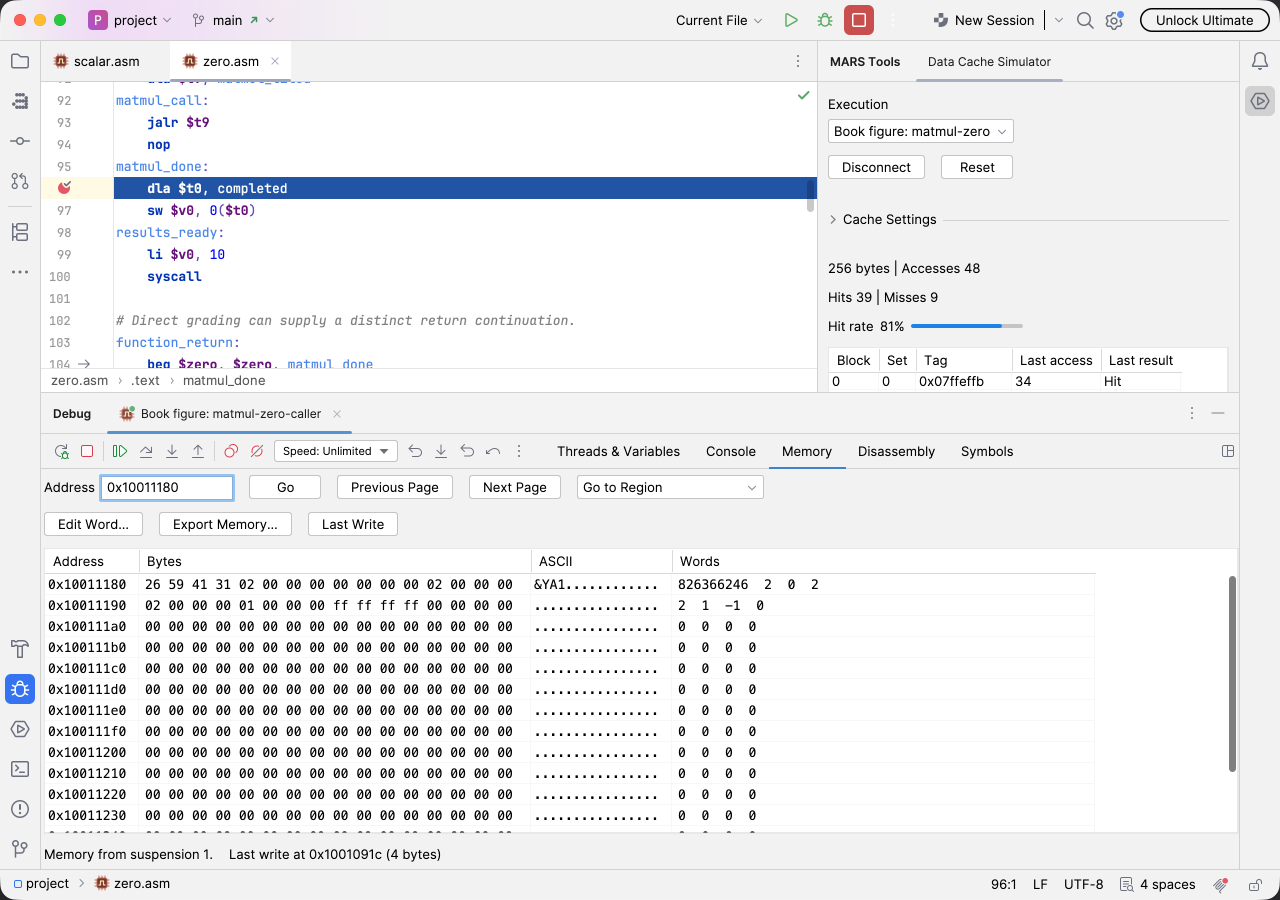
\includegraphics[width=0.84\linewidth,artifact,trim={\MARSmatmulzerocallerLeft{} \MARSmatmulzerocallerBottom{} \MARSmatmulzerocallerRight{} \MARSmatmulzerocallerTop{}},clip]{packages/022-blocked-matmul/captures/f02/caller.png}};
\begin{scope}[shift={(caller.south west)},x={($(caller.south east)-(caller.south west)$)},y={($(caller.north west)-(caller.south west)$)}]
\draw[black,line width=0.7pt] (0.194672131,0.055555556) rectangle (0.997950820,0.638888889);
\node[draw=black,fill=white,circle,inner sep=1.5pt,font=\footnotesize] at ($(0,0.638888889)+(-3mm,0)$) {4};
\end{scope}
\end{tikzpicture}
\par\smallskip
\begin{minipage}{\linewidth}
\small
\begin{enumerate}
\setlength{\itemsep}{2pt}
\setlength{\parsep}{0pt}
\item This stop follows the tiled function\textquotesingle s return. With $M=N=2$ and $K=0$, the output is nonempty even though every dot product has no terms.
\item \texttt{v0 = 4} still counts four output cells. A zero reduction dimension does not make the returned count zero.
\item The 32 selected output bytes are all zero, replacing their initial \texttt{a5 a5 5a 5a} word pattern. Empty sums must be stored as exact zero doublewords; leaving output untouched would preserve that pattern.
\item The shape words are $2,0,2,2$, method is one, and \texttt{completed} remains $-1$. The independent access history verifies no reads from either input arena. The photograph shows output state; the trace establishes that read constraint.
\end{enumerate}
\end{minipage}
\caption{Zero reduction still initializes every cell of a nonempty result.}
\label{capture:022-blocked-matmul-f02}
\label{matmul-f02}
\end{figure}
\par
